\section{Coloured Petri Nets}

To present the concepts of CPNs we use a CPN model of a distributed
two-phase commit transaction system. We use the example to give an
informal introduction to CPNs. The reader interested in the formal
definition of CPNs is referred to \cite{X}.

% modules - substitution transitions

The CPN model of the two-phase commit system is comprised of 4
\concept{modules} hierarhically organised into three
level. Figure~\ref{fig:commit} shows the top-level module which
consists of two \concept{substitution transitions} (rectchanges drawn
with \fix{double borders} representing the \figitem{Coordinator} and
the \concept{Workers} in the system. Each of the substitution
transition has an associated \concept{submodule} that model the
behaviour of the coordinator and the workers, respectively. The name
of an associated submodule is written in the reactangular tag
positioned at the bottom of the substitution transition. 

\begin{figure*}[t]
\centering
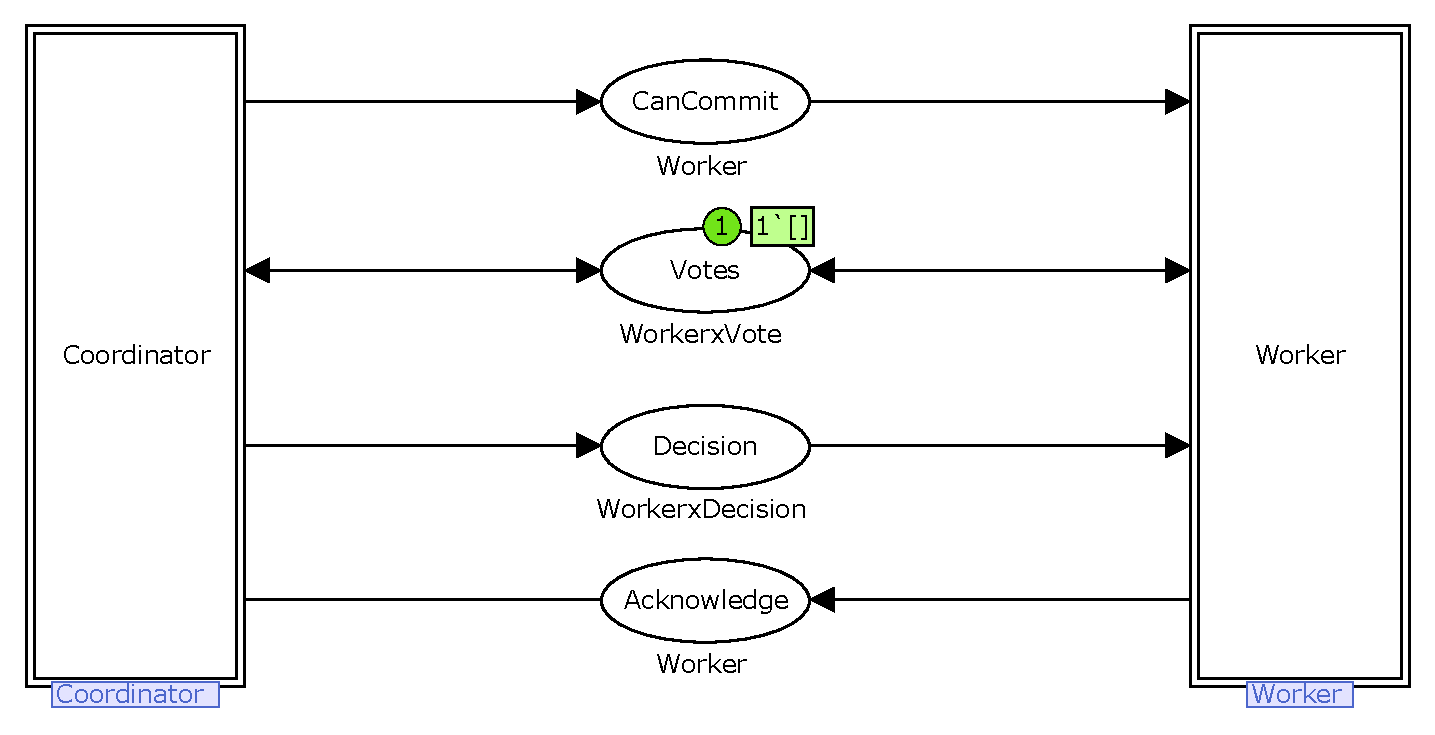
\includegraphics[scale=.5]{figures/Commit.eps}
\caption{The top-level module of the CPN model.}
\end{figure*}

% places - tokens - colours - and colour sets

The two substitution transitions are connected via directed
\concept{arcs} to the four places \figitem{CanCommit},
\figitem{Votes}, \figitem{Decision}, and \figitem{Acknowledge} (drawn
as ellipses). Places connected to substitution transition are called
\concept{socket places} and these are linked to \concept{port} places
on the associated submodules (to be explained shortly). The
coordinator and the worker interact by producing and consuming
\concept{tokens} on the places. These tokens carry data values and the
type of tokens that may reside on a place is determined by the colour
set (type) of the place which by convention is written below the
place. Figure~\ref{commitcolsets} lists the definition of the colour
sets used as colour set of the four places in
Fig.~\ref{fig:commit}. These colour sets are defined using the CPN ML
programming language.

\begin{figure}
\begin{verbatim}
val W = 2;
colset Worker = index wrk with  1..W;
colset Vote   = with Yes | No;

colset WorkerxVote = product Worker * Vote;

colset Decision        = with abort | commit;
colset WorkerxDecision = product Worker * Decision;
\end{verbatim}
\caption{Colour sets definition used in the top-level module.}
\end{figure}

The \smlcode{Worker} colour set is an indexed colour set consisting of
the values \smlcode{wrk(1),wrk(2),...,wrk(W)} where the symbolic
constant \smlcode{W} is used to denote the number of worker processes
considered. This coluor set is used to model the identity of the
worker processes in the system. The colour set \smlcode{Vote} is an
enumeration colour set containing the value \smlcode{Yes} and
\smlcode{No} is is used to model that a worked by vote yes or no to
commit the transaction. The colour set \smlcode{WorkerxVote} is a list
of products consisting of a worker and a vote. The colour set
\smlcode{Decision} is an enumration colour set used to model whether
the coordinator decides to \smlcode{abort} or \smlcode{commit} the
transaction (only if all workers vote yes will the transaction be
committed). It should be noted that in addition the type constructors
introduced above, CPN ML also supports union, lists, and record types.

% marking - tokens initial marking - current marking

The state of a CPN model (in CPN terminology called a
\concept{marking}) consists of a distribution of \concept{tokens} on
the places of the model. Each place may hold a (possibly empty)
\concept{multi-set} of tokens with data values (colours) from the
colour set of the place. The \concept{initial marking} of a place is
specified above each place (and omitted if the initial marking is the
empty multi-set). In Fig.~\ref{fig:commit} only the place
\figitem{Votes} has a non-empty initial marking which consisis of a
single token with the colour corresponding to the empty list. In CPN
ML this multi-set is written \smlcode{1`[]} specifying one
(\smlcode{1}) occurrence of (\smlcode{`}) the empty list
(\smlcode{[]}). Initially, the \concept{current marking} of a CPN
model equals the initial marking. When a a CPN model is executed
occurreces of enabled transitions consume and produce tokens on the
places which will change the \concept{current marking} of the CPN
model. The number of tokens on a place in the current marking is
indicated with a small circle positioned next to a place, and the
detail of the colour of the tokens are provided in an associated text
box. The indication of the current marking of a place is omited if
currently the place contains no tokens.
 
% coordinator  - port places

The \figitem{Coordinator} module is shown in
Fig.~\ref{fig:coordinator}. This is the submodule associated with the
\figitem{Coordinator} submodule in Fig.~\ref{fig:commit}. The places
\figitem{CanCommit}, \figitem{Votes}, \figitem{Decision}, and
\figitem{Acknowledge} are \concept{port places} as indiced by the
small \figitem{In}, \figitem{Out}, and \figitem{I/O} tags positioned
next to them. These places are linked to the accordingly named places
in the top-level module (Fig.~\ref{fig:commit}) via a
\concept{port-socket assosiation} which implies that any tokens
added/removed from a port places by transitions in the
\concept{Cooordinator} module will also be reflected in the marking of
the associated socket places in the top-level module. The place
\figitem{CanCommit} is an output port places which means that this
submodle will only produce tokens on this place, and place
\figitem{Acknowledge} is an input port place which means that the
module will only consume tokens from this place. Place \figitem{Votes}
is an input/output port place which means that this module may both
produce and consume tokens on/from this place. 

\begin{figure}[t]
\centering
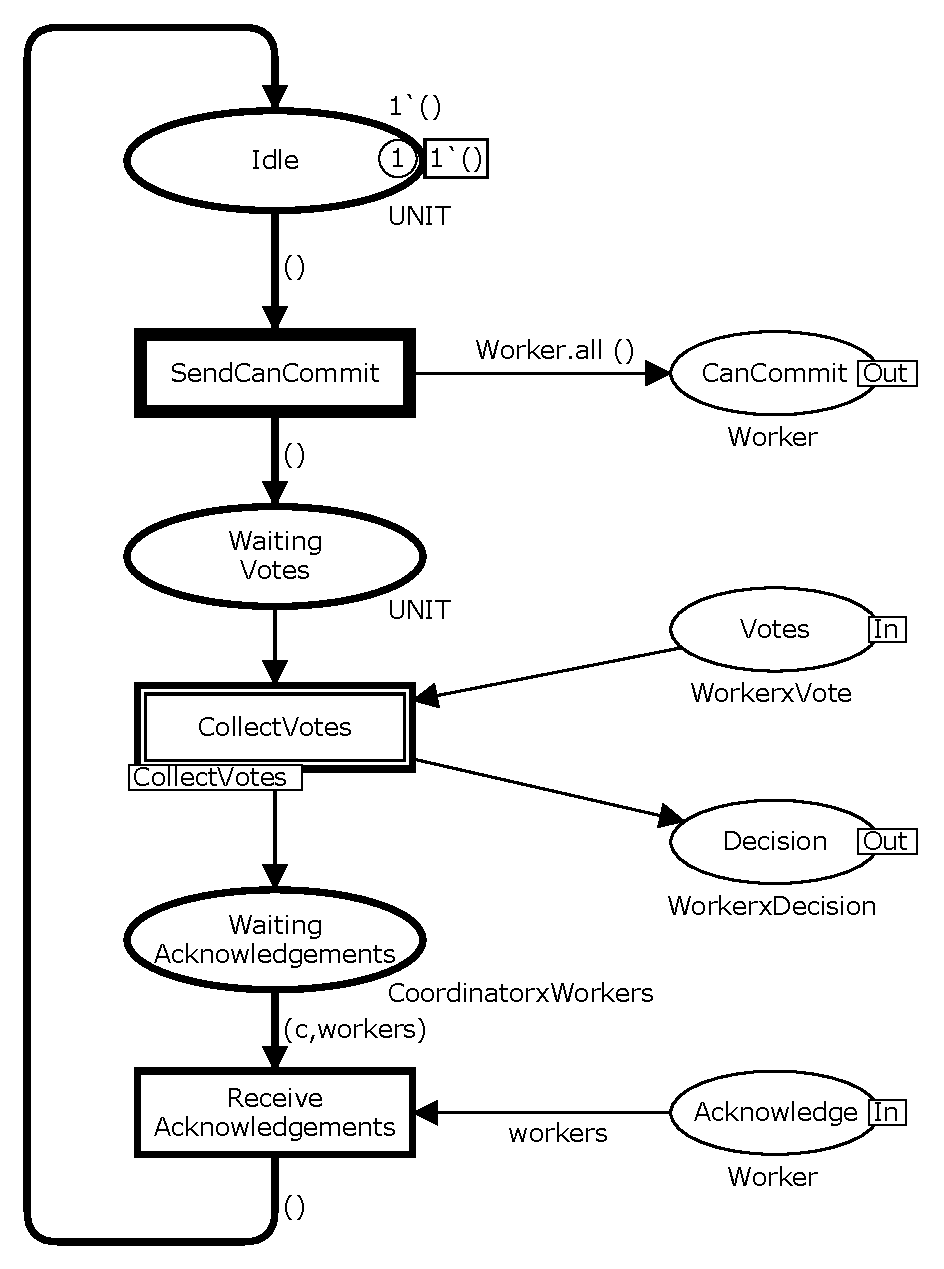
\includegraphics[width=\columnwidth]{figures/Coordinator.eps}
\caption{The Coordinator module.}
\end{figure}

The places \figitem{Idle}, \figitem{WaitingVotes}, and
\figitem{WaitingAcknowledgement} are used to model the states that the
coordinator goes throigh when executing the two-phase commit
protocol. The places \figitem{Idle} and \figitem{WaitingVotes} have the
colour set \smlcode{UNIT} containing just a single value \smlcode{()}
denoted unit. Initially, the coordinator is in an idle state as
modelled by the initial marking of place \figitem{Coordinator}. The
transitions \figitem{SendCanCommit}, \figitem{CollectVotes}, and
\figitem{ReceiveAcknowledge} models the event/actions that cause the
coordinator to change state. The coordinator will first send a message
to each worker asking whether they can commit the transaction; then
the coordinator will collect the votes from all workers and then send
a decision to each working indicating whether the transaction is to be
committed or not. Finally, the coordinator will receive and
acknowledgement from each worker that they have received the
deceision.  It should be noted that \figitem{CollectVotes} is a
substituion transition which means that the details of how the
coordinator collects votes is modelled by the associated
\figitem{CollectVotes} submodule. This illustrates that it is possible
to mix the use of ordinary and substitution transitions within a
module.

% basic enabling and occurrences

In the current marking shown in Fig.~\ref{fig:coordinator} only the
transition \figitem{SendCanCommit} is enabled as indicated by the
thick border of that transition. The requirement for a transition to
be \concept{enabled} is determined from the \concept{arc expressions}
associated with the incoming arcs of the transition. In this case,
there is only a single incoming arc from place \figitem{Idle}
containing the expression \smlcode{()}. This expression specifies that
for \figitem{SendCanCommit} to be enabled, there must be at least one
\smlcode{()}-token present on \smlcode{Idle}. When the
\smlcode{SendCanCommit} transition \concept{occurs} it will consume a
\smlcode{()}-token from place \smlcode{Idle} and it will produce
tokens on place connected to output arcs as determing by evaluating
the arc expressions of the corresponding arcs. In this case, the
expression \smlcode{()} on the arc to \smlcode{WaitingVotes} evaluates
to a single \smlcode{()}-token while the expression \smlcode{Workers}
evaluates to the set of all workers. 

Figure~\ref{fig:sendcancommit} shows the marking of the sourrounding
places of transition \figitem{SendCanCommit}. It can be seen that the
place \smlcode{CanCommit} contains two tokens - one of each worker in
the system - representing messages going to the two worker
processes. The coordinator has now enetered a state in which it is
waiting to collect the votes from the worker processes.

TODO: ADD THE FIGURE

% comparison to low-level nets

By setting the symbolic constant \smlcode{W} (see
Fig.~\ref{fig:coloursets}) we can easily configure to model to handle,
e.g., five workers. With ordinary Petri nets we would have had to
create a copy of the \figitem{CanCommit} place for each worker. In
particular, we would have to make changes to the net structure
(places, transitions, arcs) when changing the number of workers. This
shows that CPNs provides a means for easily creating parametriseble
models and also that it enables more compact modelling as we only need
a single instance of the \figitem{CanCommit} place in order to
accomodate any finite number of workers.

%\com{Maybe we could have shown
%  the corresponding fragment as a Place/Transition net? In this case we need more places - when we get to the worker we could also need to duplicate transition as per bindings}

% worker process - and binding and binding elements.

Figure~\ref{fig:worker} shows the \figitem{Worker} module which is the
submodule of the \figitem{Workers} substitution transition in
Fig.~\ref{fig:commit}. The place \figitem{CanCommit}, \figitem{Votes},
\figitem{Decision}, and \figitem{Acknowledge} constitute the port
places of this module and are linked to the accordingly named socket
places in Fig.~\ref{fig:commit}. The places \figitem{Idle} and
\figitem{Waiting} models the two main states of worker processes. Each
of these places have the colour set \smlcode{Worker} and the idea is
that when there is a token with colour \smlcode{wrk(i)} on, e.g., the
place \figitem{Idle} then this represent that the i'th worker is in
state idle. This makes it possible to model the state of all workers
in a compact manner without having to have a place for each
worker. Initially, all workers are in the idle state as represented by
correspondings tokens on place \figitem{Idle} in the initial
marking. The transition \figitem{ReceiveCanCommit} models the
reception of can commit messages from the coordinator and the sending
of a vote. The transition \figitem{ReceiveDecision} models the
reception of a decision message from the coordinator and then sending
of an acknowledment. 


The current marking of place \figitem{CanCommit} is \smlcode{1`wrk(1)
  ++ 1`wrk(2)} corresponding a marking where the coordinator has sent
a can commit message to each worker. The thick border of transition
\figitem{ReceiveCanCommit} indicates that this transition is enabled
in the current marking depicted in the figure. The arc expressions on
the sourrounding arcs of the \figitem{ReceiveCanCommit} transition is
more complex than the arc expressions of the \figitem{SendCanCommit}
transition in the \figitem{Coordinator} module considered earlier in
that they contain the \smlcode{free variables} \smlcode{w} and
\smlcode{votes} defined in Fig.~\ref{fig:variables}. This means that
in order to talk about the enabling and occurrence of transition
\smlcode{ReceiveCanCommit} we need to assign values to these variables
in order to evaluate the input and output arc expression. This is done
by creating a \concept{binding} which associates a value to each of
the free variables occurring in the arx expression of the
transitions. As \smlcode{w} is of type \smlcode{Worker} and
\smlcode{vote} is of type \smlcode{Decision} this gives the following
four possible bindings reflecting that each of the two workers may
vote yes or no to committing the transactions:

\begin{eqnarray*}
b_{1Y} & = & \langle \smlcode{w} = \smlcode{wrk(1)}, \smlcode{vote} = \smlcode{Yes} \rangle \\
b_{1N} & = & \langle \smlcode{w} = \smlcode{wrk(1)}, \smlcode{vote} = \smlcode{No} \rangle \\
b_{2Y} & = & \langle \smlcode{w} = \smlcode{wrk(2)}, \smlcode{vote} = \smlcode{Yes} \rangle \\
b_{2N} & = & \langle \smlcode{w} = \smlcode{wrk(2)}, \smlcode{vote} = \smlcode{No} \rangle
\end{eqnarray*}

A binding of a transition is then enabled if evaluating each input arc
expression in the binding results in a multi-set of tokens which is
contained in the multi-set of tokens present on the corresponding
input place. Considering, the binding $b_{1Y}$ then evaluting the
input arc expression \smlcode{w} on the input arc from \smlcode{Idle}
results in the multi-set containing a single token with the colour
\smlcode{wrk(1)} which is contained in the multi-set of tokens present
on place \figitem{Idle} in the marking depicted in
Fig.~\ref{fig:worker}. Similarly for the input arc expression on the
arc from place \figitem{CanCommit}. This means that binding $b_{1Y}$
is enabled an may occur. In fact, all the four bindings listed above
is enabled in the marking shown in Fig.~\ref{fig:commit}. 

% ocurrence and more complicated evaluation

Bindings can be considered different modes in which a transition may
occur. The tokens produced on output places when an transition occur
in an enabled binding is determined by evaluating the output arc
expression of the transition in the given binding. Consider again the
binding element $b_{1Y}$. The output arc expression \smlcode{(w,vote)}
will evaluate to \smlcode{wrk(1),Yes} and this token will be added to
place \smlcode{Votes} to inform the coordinator that worker one votes
yes to committing the transaction. The arc expression on the arc from
\figitem{ReceiveCanCommit} to \figitem{Waiting} is an if-then-else
expression which in the binding $b_{1Y}$ will evaluate to the
multi-set $1`wrk(1)$ which will then be added to the tokens on place
\figitem{Waiting}. The if-then-else expression on the arc from
\figitem{ReceiveCanCommit} evaluates to the \smlcode{empty} multi-set
and hence no tokens will be added to place \figitem{Idle} in this
case. Figure~X shows the marking resulting from an occurrence of the
$b_{1Y}$ binding.

The occurrence of the binding $b_{1N}$ representing that worker one
votes no would have the effect of removing a wrk(1) token from
\figitem{Idle}, and adding no tokens to place \figitem{Waiting} and
adding one wrk(1) token to place \figitem{Idle}. This models the fact
that if a worker votes no to committing the transaction it goes back
to idle whereas if it vores yes, then it will go to waiting to be
informed about whether the transaction is to be committed or not
(recall that this is a distributed system so one worker cannot know
what other workers have voted). Above we have considered relativly
simple arc expression but the arc expression of a transition can be
any expression that can be written in Standard ML as long as it has a
type that matches the corresponding place. In particular, arc
expressions may apply functions including higher-order functions.

It follows from the above that the all of the four bindings of
transition \figitem{ReceiveCanCommit} were enabled. Furthermore,
enabled bindings may be \concept{concurrently enabled} if each binding
can get its tokens from input place independely of other bindings in
the set. As an example, the two bindings $b_{1Y}$ and $b_{2Y}$ because
each binding can gets its token from the input place without competing
with each other. This reflects that the workers are executing
concurrently and may simulranous send a vote back to the
coordinator. In contrast, the two bindings $b_{1Y}$ and $b_{1N}$ are
nor concurrent but in \concept{conflict} because they each need, e.g.,
the single wrk(1) token on \figitem{Idle} (and in fact also the single
wrk(1) token on place \figitem{CanCommit}. THe notion of concurrency
and conflict of binding extends to also span to bindings of different
transitions.

%% here we could perhaps talk breifly about time.
